\ExerciseChapter{一般线性模型}

\label{chapter:3}

\section{往年题}

\subsection{单项选择题}

\Needspace{7\baselineskip}\subsubsection*{共用资料：减肥训练与基线不均衡}

在一个减肥训练班（训练方法为控制饮食与锻炼）中招募志愿者服用减肥药，志愿者和其他人都继续饮食控制与锻炼。用试验前后体重减少量评价疗效；研究人员发现服药志愿者通常比非志愿者更肥胖，两个组的基线不均衡。


\par\addvspace{6pt}\noindent\begin{minipage}{\linewidth}

\Question{E14-1}{调整不均衡的基线}

研究者希望控制基线不均衡可能带来的混杂效应,宜使用何种统计方法?


\begin{choices}

\item 配对t检验

\item 单因素方差分析

\item 线性回归

\item GLM

\item 非条件logistic回归

\end{choices}

\end{minipage}\par\vspace{4pt}

\par\addvspace{6pt}\noindent\begin{minipage}{\linewidth}

\Question{E14-2}{基线与处理的交互}

如果基线体重和分组变量存在交互作用,则


\begin{choices}

\item 难以判定药物减肥效果

\item 需进一步做成组设计均数比较的t检验

\item 需计算调整后的OR值

\item 可以计算偏相关系数做疗效判断

\item 可以计算标准化回归系数做进一步比较

\end{choices}

\end{minipage}\par\vspace{4pt}

\par\addvspace{6pt}\noindent\begin{minipage}{\linewidth}

\Question{E14-3}{无交互后的疗效评价}

如果基线体重和分组变量不存在交互作用,则


\begin{choices}

\item 可以判定减肥药无效

\item 无论基线体重与体重减少量是否有线性关系,都可以进一步评价药物的减肥效果

\item 如果基线体重与体重减少量无线性关系,可以认为减肥药有效

\item 可以直接做单因素方差分析

\item 以MH卡方检验或logistic模型分析

\end{choices}

\end{minipage}\par\vspace{4pt}

\par\addvspace{6pt}\noindent\begin{minipage}{\linewidth}

\Question{E14-4}{散点图与表观药效}

如果下图是数据的散点图,则最可能的结论是

\begin{center}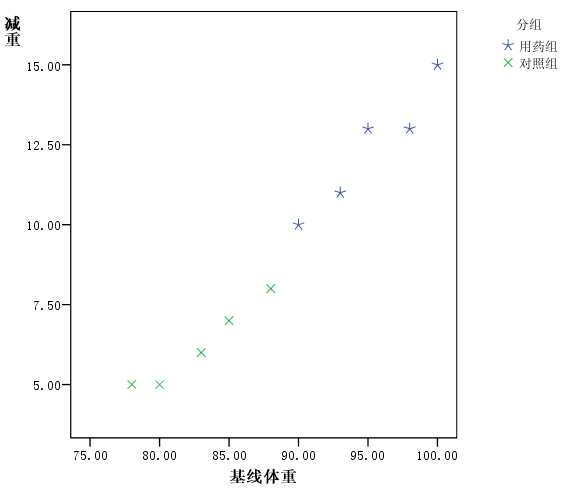
\includegraphics[width=.80\linewidth]{assets/weight2014.png}\end{center}


\begin{choices}

\item 两组基线体重均衡

\item 基线体重与用药存在交互作用

\item 基线体重与减重的分组回归线平行且重合

\item 成组比较(减重) 结果为两组差异无统计学意义

\item 减肥药有效

\end{choices}

\end{minipage}\par\vspace{4pt}

\par\addvspace{6pt}\noindent\begin{minipage}{\linewidth}

\Question{E14-5}{将连续疗效二分类}

如果研究者以体重减少5kg为疗效判断指标,将结果变量设为有效和无效并使用logistic回归分析,则以下错误的说法是


\begin{choices}

\item 损失了数据信息,降低了检验效能

\item 如果发现药物有效,同时也可确定药物的临床使用价值

\item 如果没有其他混杂因素,可以同时计算 RR和OR

\item 可以用有效和无效分组,比较两组人的平均体重,如果有效组平均体重高于无效组,则说明减肥药对胖人有效

\item 可以考察基线体重和分组变量间的交互作用

\end{choices}

\end{minipage}\par\vspace{4pt}

\Needspace{7\baselineskip}\subsubsection*{共用资料：两所医院的护理量与新生儿死亡}

医院和护理按表中1/2编码，响应为死亡1、存活0。下表给出4个Logistic模型的原输出；P显示0.000表示小于显示精度，不代表概率严格为0。

\begin{center}\small\setlength{\tabcolsep}{3.5pt}\renewcommand{\arraystretch}{1.18}\begin{tabular}{@{}lrrrr@{}}
\toprule
医院 & 护理量 & 死亡 & 存活 & 死亡率\% \\
\midrule

A（1） & 少（1） & 3 & 176 & 1.676 \\
A（1） & 多（2） & 4 & 293 & 1.347 \\
B（2） & 少（1） & 17 & 197 & 7.944 \\
B（2） & 多（2） & 1 & 23 & 4.0 \\
\bottomrule\end{tabular}\end{center}

\begin{center}\small\setlength{\tabcolsep}{3.5pt}\renewcommand{\arraystretch}{1.18}\begin{tabular}{@{}lrrrrrrr@{}}
\toprule
模型 & 变量 & B & SE & Wald & df & P & Exp(B) \\
\midrule

1 & hospital & 2.085 & 1.705 & 1.495 & 1 & 0.221 & 8.048 \\
1 & nurse & 0.241 & 1.865 & 0.017 & 1 & 0.897 & 1.273 \\
1 & hospital×nurse & -0.463 & 1.304 & 0.126 & 1 & 0.722 & 0.629 \\
1 & 截距 & -5.935 & 2.782 & 4.553 & 1 & 0.033 & 0.003 \\
2 & hospital & 1.507 & 0.528 & 8.159 & 1 & 0.004 & 4.515 \\
2 & nurse & -0.395 & 0.592 & 0.445 & 1 & 0.505 & 0.674 \\
2 & 截距 & -5.089 & 1.423 & 12.78 & 1 & 0.0 & 0.006 \\
3 & hospital & 1.701 & 0.453 & 14.115 & 1 & 0.0 & 5.482 \\
3 & 截距 & -5.906 & 0.8 & 54.499 & 1 & 0.0 & 0.003 \\
4 & nurse & -1.22 & 0.506 & 5.822 & 1 & 0.016 & 0.295 \\
4 & 截距 & -1.705 & 0.643 & 7.027 & 1 & 0.008 & 0.182 \\
\bottomrule\end{tabular}\end{center}


\par\addvspace{6pt}\noindent\begin{minipage}{\linewidth}

\Question{E14-6}{护理量与医院的调整分析}

根据统计结果,新生儿死亡的影响因素是


\begin{choices}

\item 仅医院原因

\item 仅护理量原因

\item 医院原因和护理量二者均是影响因素

\item 不同护理量下,A,B医院的影响不同

\item 无法判断

\end{choices}

\end{minipage}\par\vspace{4pt}

\par\addvspace{6pt}\noindent\begin{minipage}{\linewidth}

\Question{E14-7}{未调整的护理OR}

如果忽略医院不同的影响做单因素分析,较高护理量对较低护理量的OR是


\begin{choices}

\item 0

\item 0.295

\item 0.674

\item 1

\item 1.273

\end{choices}

\end{minipage}\par\vspace{4pt}

\par\addvspace{6pt}\noindent\begin{minipage}{\linewidth}

\Question{E14-8}{最终医院OR}

根据最终统计结果,B医院对A医院的OR是


\begin{choices}

\item 0

\item 1

\item 4.5

\item 5.5

\item 8.0

\end{choices}

\end{minipage}\par\vspace{4pt}

\par\addvspace{6pt}\noindent\begin{minipage}{\linewidth}

\Question{E14-9}{被删除项的模型OR}

根据最终统计结果,较高护理量对较低护理量的OR是


\begin{choices}

\item 0

\item 0.295

\item 0.674

\item 1

\item 1.273

\end{choices}

\end{minipage}\par\vspace{4pt}

\par\addvspace{6pt}\noindent\begin{minipage}{\linewidth}

\Question{E14-10}{医院间的风险比}

根据最终统计结果,B医院对A医院的RR是


\begin{choices}

\item 1.1

\item 4.5

\item 5.1

\item 5.5

\item 8.0

\end{choices}

\end{minipage}\par\vspace{4pt}

\par\addvspace{6pt}\noindent\begin{minipage}{\linewidth}

\Question{E14-11}{三个OR的组合}

某药效临床试验,研究对象分低龄和高龄两组随机分配入用药组和安慰剂组,使用logistic model,以高龄和安慰剂为参照,得到年龄的OR=2,药物的OR=5,年龄和药物的交互作用为0.8,则低龄用药组对高龄安慰剂组的OR是


\begin{choices}

\item 6.2

\item 7.8

\item 8

\item 10

\item 10.8

\end{choices}

\end{minipage}\par\vspace{4pt}

\par\addvspace{6pt}\noindent\begin{minipage}{\linewidth}

\Question{E14-13}{一般线性模型与参照类别}

关于GLM,以下判断正确的是


\begin{choices}

\item 不要求因变量服从正态分布

\item 要求自变量互相独立

\item 对于有交互作用的模型,可以在估计交互作用后评价主效应

\item 对于无交互作用模型,可以直接做单因素方差分析

\item 可以任意指定某分类变量中某类的主效应参数(回归系数)为0

\end{choices}

\end{minipage}\par\vspace{4pt}

\Needspace{7\baselineskip}\subsubsection*{共用资料：旧题文献2与Framingham模型}

原题引用《多元线性回归\ldots\ldots》及Framingham心脏病研究的表1、方程；该原文未随本题库提供。现有``生命质量影响因素''是另一篇2018年文献，不能代替。以下保留原题，涉及具体数值与文章原句的答案须等待原文核验。


\par\addvspace{6pt}\noindent\begin{minipage}{\linewidth}

\Question{E14-18}{由原文方程计算风险}

根据表1结果,45岁,女性,SBP\textless22kPa,其冠心病发病的概率是


\begin{choices}

\item 0.0613

\item 0.0277

\item 0.1273

\item 0.1680

\item 尚无法判断

\end{choices}

\end{minipage}\par\vspace{4pt}

\Needspace{7\baselineskip}\subsubsection*{共用资料：BMI与非吸烟女性肺癌}

上海市肿瘤登记收集1992年2月1日至1993年底的女性肺癌新病例649例，年龄35---69岁；73\%由病理或细胞学确诊，其余经胸部影像。按病例年龄分布，以5岁为组作频数匹配，在市区人群中随机抽取健康对照675例。非吸烟病例、对照分别为504、601例。对非吸烟者拟合多变量非条件Logistic模型，调整烹调油烟、用油类型、被动吸烟、饮茶、肺结核、家族史、月经生育等因素；下表为两个调整层次的结果。原结论：``体质指数可能是非吸烟女性肺癌的危险因素之一。''

\begin{center}\small\setlength{\tabcolsep}{3.5pt}\renewcommand{\arraystretch}{1.18}\begin{tabular}{@{}lrrrrr@{}}
\toprule
BMI组 & 病例/对照 & ORI & 95\% CII & ORII & 95\% CIII \\
\midrule

\(\ge\) 25.15 & 94/152 & 1 & --- & 1 & --- \\
22.86---25.14 & 103/159 & 1.017 & 0.706---1.464 & 1.021 & 0.707---1.473 \\
20.96---22.85 & 129/140 & 1.399 & 0.976---2.006 & 1.498 & 0.971---2.012 \\
\textless20.96 & 176/150 & 1.793 & 1.268---2.536 & 1.794 & 1.263---2.548 \\
\bottomrule\end{tabular}\end{center}

两个模型的趋势检验均报告 \(P=0.0002\)。


\par\addvspace{6pt}\noindent\begin{minipage}{\linewidth}

\Question{E14-22}{病例对照设计}

本研究属于


\begin{choices}

\item 横断面调查研究

\item 病例对照研究

\item 队列研究

\item 社区干预研究

\item 随机对照临床试验

\end{choices}

\end{minipage}\par\vspace{4pt}

\par\addvspace{6pt}\noindent\begin{minipage}{\linewidth}

\Question{E14-23}{病例对照研究的实施难点}

按此研究设计,在操作上最难做到的是


\begin{choices}

\item 获得癌症病人资料

\item 获得对照组人群资料

\item 问卷调查

\item BMI测试

\item 统计分析

\end{choices}

\end{minipage}\par\vspace{4pt}

\par\addvspace{6pt}\noindent\begin{minipage}{\linewidth}

\Question{E14-24}{表内数字核查}

此研究中肯定存在的问题有


\begin{choices}

\item 统计数字有误

\item 假设检验有误

\item OR计算有误

\item 资料获取方法有误

\item 模型选择有误

\end{choices}

\end{minipage}\par\vspace{4pt}

\par\addvspace{6pt}\noindent\begin{minipage}{\linewidth}

\Question{E17-M6}{有序分类自变量的分析}

当Y为数值变量,X为有序多分类变量,则以下正确的说法是


\begin{choices}

\item 使用单因素方差分析最优

\item 可以直接进行多次t检验

\item 使用等级相关分析最优

\item 使用GLM进行分析最优

\item 如果LINE假设成立，宜用线性回归分析，模型假设检验的自由度为1。

\end{choices}

\end{minipage}\par\vspace{4pt}

\par\addvspace{6pt}\noindent\begin{minipage}{\linewidth}

\Question{E17-M19}{温度与催化剂的关系}

欲考察某化学反应条件(温度、催化剂)与底物浓度(变化)的关系,数据分析宜使用


\begin{choices}

\item 分组散点图。

\item 边际均数图。

\item 偏回归图。

\item QQ图。

\item 残差分布图。

\end{choices}

\end{minipage}\par\vspace{4pt}

\Needspace{7\baselineskip}\subsubsection*{共用资料：减肥训练与基线不均衡}

在一个减肥训练班（训练方法为控制饮食与锻炼）中招募志愿者服用减肥药，志愿者和其他人都继续饮食控制与锻炼。用试验前后体重减少量评价疗效；研究人员发现服药志愿者通常比非志愿者更肥胖，两个组的基线不均衡。


\par\addvspace{6pt}\noindent\begin{minipage}{\linewidth}

\Question{E17-C1}{基线不均衡还能否分析}

如果服药组与对照组的体重基线不均衡,则本研究


\begin{choices}

\item 无法回答药物是否有效问题

\item 使用GLM模型可以消除体重不均衡因素,回答药物是否有效问题

\item 不妨使用t 检验做成组比较

\item 在一定情况下可以回答药物是否有效问题

\item 因为没有随机入组,本试验无效

\end{choices}

\end{minipage}\par\vspace{4pt}

\par\addvspace{6pt}\noindent\begin{minipage}{\linewidth}

\Question{E17-C2}{药效依赖基线水平}

如果基线体重和分组变量存在交互作用,则


\begin{choices}

\item 可以计算标准化回归系数做进一步比较

\item 需进一步做成组设计均数比较的t检验

\item 药效大小与体重有关

\item 可以计算偏相关系数做疗效判断

\item 可以判定药物减肥有效

\end{choices}

\end{minipage}\par\vspace{4pt}

\par\addvspace{6pt}\noindent\begin{minipage}{\linewidth}

\Question{E17-C3}{共同斜率模型的下一步}

如果基线体重和分组变量不存在交互作用,则


\begin{choices}

\item 即可判定减肥药有效

\item 可以通过进一步分析得出药物是否有效的结论

\item 如果基线体重与体重减少量无线性关系,可以认为减肥药有效

\item 如果基线体重与体重减少量有线性关系,亦难评价减肥药是否有效

\item 即可做单因素方差分析来进一步判定

\end{choices}

\end{minipage}\par\vspace{4pt}

\par\addvspace{6pt}\noindent\begin{minipage}{\linewidth}

\Question{E17-C4}{重叠趋势与基线混杂}

如果下图是数据的散点图,则最可能的结论是

\begin{center}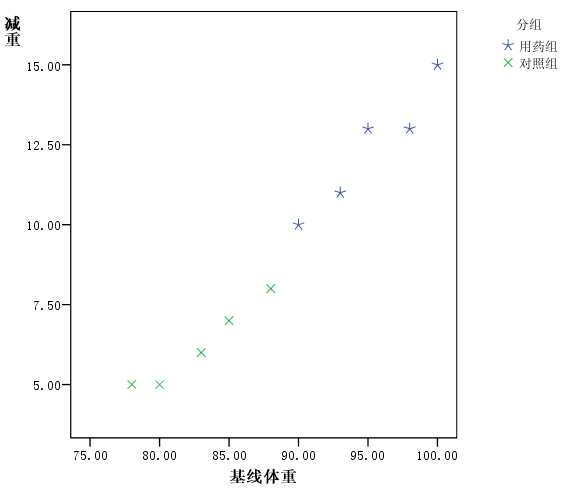
\includegraphics[width=.80\linewidth]{assets/weight2017.png}\end{center}


\begin{choices}

\item 两组基线体重均衡

\item 基线体重与分组变量存在交互作用

\item 减肥药无效

\item 基线体重与减重无线性关系

\item 成组比较(减重) 结果为两组差异无统计学意义

\end{choices}

\end{minipage}\par\vspace{4pt}

\par\addvspace{6pt}\noindent\begin{minipage}{\linewidth}

\Question{E17-C5}{基线均衡后的分析选择}

如果两组基线体重均衡,则以下错误的说法是


\begin{choices}

\item 无把握判断减肥药是否有效

\item 可以科学判断训练方法是否有效

\item 可以使用t检验

\item 必须基线体重为协变量建立GLM

\item 可以使用方差分析

\end{choices}

\end{minipage}\par\vspace{4pt}

\Needspace{7\baselineskip}\subsubsection*{共用资料：急诊就诊量与气象要素}

阅读随包的《急诊就诊量与气象要素的相关性分析》（费敏，2008）。研究分析2005---2006连续730天数据，报告急诊199649人次、日均274.5人次；7月最高、2月最低。文中写采用post hoc检验。回归从9个气象变量中筛出以下4项：

\begin{center}\small\setlength{\tabcolsep}{3.5pt}\renewcommand{\arraystretch}{1.18}\begin{tabular}{@{}lrrrr@{}}
\toprule
变量 & B & SE & 标准化\(\beta\) & P \\
\midrule

平均相对湿度 & 1.011 & 0.159 & 0.244 & \textless.001 \\
最高气温 & 1.126 & 0.546 & 0.212 & \textless.05 \\
最低气温 & 2.2 & 0.591 & 0.378 & \textless.001 \\
最大风速 & -0.606 & 0.091 & -0.207 & \textless.001 \\
\bottomrule\end{tabular}\end{center}

给出的预测公式截距为285.481。讨论中认为春节期间停工休息可能减少意外就诊，也讨论高温和低温均可能增加急症。文中未给出本模型的 \(R^2\)、时间序列残差或共线性诊断；所引用的84\%与44\%来自别人的研究。


\par\addvspace{6pt}\noindent\begin{minipage}{\linewidth}

\Question{E17-L1}{月份均数的事后比较}

7月份和2月份日平均就诊人次与其他月份相比差异有统计学意义,作者最可能使用的统计方法是


\begin{choices}

\item GLM

\item t检验

\item 线性回归

\item 方差分析后的多重比较 post-hoc

\item 非参数检验

\end{choices}

\end{minipage}\par\vspace{4pt}

\par\addvspace{6pt}\noindent\begin{minipage}{\linewidth}

\Question{E17-L5}{0.0613对应什么人群}

依照Framingham心脏病研究的回归方程,0.0613是指


\begin{choices}

\item 各自变量为均数时的发病率

\item 人群基线发病率

\item 45岁女性收缩压小于22者发病率

\item 血压正常者平均发病率

\item 61岁组平均发病率

\end{choices}

\end{minipage}\par\vspace{4pt}

\par\addvspace{6pt}\noindent\begin{minipage}{\linewidth}

\Question{E21-13}{含交互模型的自由度}

GLM的交互作用模型,自变量为一个数值变量和一个4分类变量,则模型误差的自由度是


\begin{choices}

\item n-5

\item n-6

\item n-7

\item n-8

\item n-9

\end{choices}

\end{minipage}\par\vspace{4pt}

\par\addvspace{6pt}\noindent\begin{minipage}{\linewidth}

\Question{E21-14}{R公式与层次原则}

按R公式语法，下列哪些模型符合层次原则？

I. \texttt{y\ \textasciitilde{}\ x1\ +\ x2\ +\ x3\ +\ x1*x2*x3}

\begin{enumerate}
\def\labelenumi{\Roman{enumi}.}
\setcounter{enumi}{1}
\item
  \texttt{y\ \textasciitilde{}\ x1\ +\ x2\ +\ x3\ +\ x1*x2\ +\ x2*x3\ +\ x1*x2*x3}
\item
  \texttt{y\ \textasciitilde{}\ x1\ +\ x2\ +\ x3\ +\ x1*x2*x3}
\end{enumerate}

三个公式按回忆稿原样保留（I与III相同）。


\begin{choices}

\item I

\item II

\item III

\item I\&II

\item I\&II\&III

\end{choices}

\end{minipage}\par\vspace{4pt}

\par\addvspace{6pt}\noindent\begin{minipage}{\linewidth}

\Question{E21-15}{aov的顺序平方和}

关于aov()函数,正确的说法有 I、aov()函数对交互作用的检验与自变量的顺序有关 II、aov()函数对主效应的检验与自变量的顺序有关 III、aov()函数可以用于协方差矩阵的球形检验


\begin{choices}

\item I

\item II

\item III

\item I\&II

\item I\&II\&III

\end{choices}

\end{minipage}\par\vspace{4pt}

\Needspace{7\baselineskip}\subsubsection*{共用资料：减肥训练与基线不均衡}

在一个减肥训练班（训练方法为控制饮食与锻炼）中招募志愿者服用减肥药，志愿者和其他人都继续饮食控制与锻炼。用试验前后体重减少量评价疗效；研究人员发现服药志愿者通常比非志愿者更肥胖，两个组的基线不均衡。


\par\addvspace{6pt}\noindent\begin{minipage}{\linewidth}

\Question{E21-21}{基线不均衡还能否分析}

如果服药组与对照组的体重基线不均衡,则本研究


\begin{choices}

\item 无法回答药物是否有效问题

\item 使用GLM模型可以消除体重不均衡因素,回答药物是否有效问题

\item 不妨使用t 检验做成组比较

\item 在一定情况下可以回答药物是否有效问题

\item 因为没有随机入组,本试验无效

\end{choices}

\end{minipage}\par\vspace{4pt}

\par\addvspace{6pt}\noindent\begin{minipage}{\linewidth}

\Question{E21-22}{药效依赖基线水平}

如果基线体重和分组变量存在交互作用,则


\begin{choices}

\item 可以计算标准化回归系数做进一步比较

\item 需进一步做成组设计均数比较的t检验

\item 药效大小与体重有关

\item 可以计算偏相关系数做疗效判断

\item 可以判定药物减肥有效

\end{choices}

\end{minipage}\par\vspace{4pt}

\par\addvspace{6pt}\noindent\begin{minipage}{\linewidth}

\Question{E21-23}{共同斜率模型的下一步}

如果基线体重和分组变量不存在交互作用,则


\begin{choices}

\item 即可判定减肥药有效

\item 可以通过进一步分析得出药物是否有效的结论

\item 如果基线体重与体重减少量无线性关系,可以认为减肥药有效

\item 如果基线体重与体重减少量有线性关系,亦难评价减肥药是否有效

\item 即可做单因素方差分析来进一步判定

\end{choices}

\end{minipage}\par\vspace{4pt}

\par\addvspace{6pt}\noindent\begin{minipage}{\linewidth}

\Question{E21-24}{重叠趋势与基线混杂}

如果下图是数据散点图，则最可能的结论是：

\begin{center}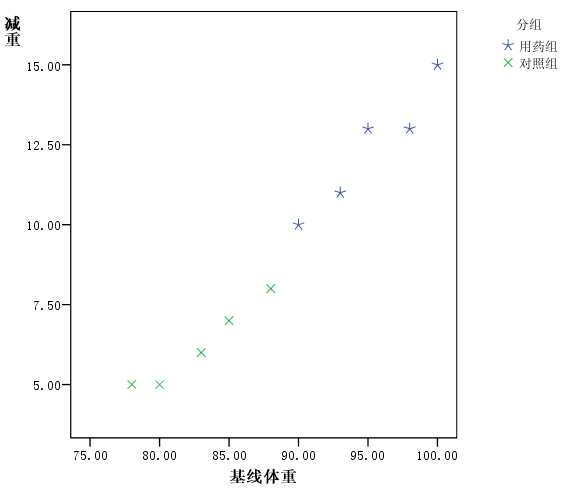
\includegraphics[width=.80\linewidth]{assets/weight2021.png}\end{center}


\begin{choices}

\item 两组基线体重均衡

\item 基线体重与分组变量存在交互作用

\item 减肥药无效

\item 基线体重与减重无线性关系

\item 成组比较(减重) 结果为两组差异无统计学意义

\end{choices}

\end{minipage}\par\vspace{4pt}

\par\addvspace{6pt}\noindent\begin{minipage}{\linewidth}

\Question{E21-25}{设计阶段的混杂控制}

这个研究给你哪些启发？

I. 只要一项基线指标均衡，就一定不存在混杂。

\begin{enumerate}
\def\labelenumi{\Roman{enumi}.}
\setcounter{enumi}{1}
\item
  组间检验不显著就证明处理完全无效。
\item
  设计阶段未考虑混杂，可能无法回答研究者关心的问题。
\end{enumerate}


\begin{choices}

\item I

\item II

\item III

\item I\&II

\item I\&II\&III

\end{choices}

\end{minipage}\par\vspace{4pt}

\par\addvspace{6pt}\noindent\begin{minipage}{\linewidth}

\Question{E21-8}{一般线性模型的组成}

一个连续结局、一个二分类因素和一个数值协变量，无交互的含截距一般线性模型可写为：


\begin{choices}

\item \(E(Y\mid X,G)=\beta_0+\beta_X X+\beta_G G\)。

\item \(Y\)必须与\(X\)相互独立。

\item 必须省略截距。

\item 必须将连续结局先二分类。

\item 无需任何关于误差和设计的条件。

\end{choices}

\end{minipage}\par\vspace{4pt}

\par\addvspace{6pt}\noindent\begin{minipage}{\linewidth}

\Question{E21-11}{交互模型的层次性}

若模型保留 \(X_1X_2\) 交互项，通常应同时保留：


\begin{choices}

\item 仅截距。

\item X1与X2两个低阶主效应。

\item 只保留P值较小的一个主效应。

\item 删除全部主效应。

\item 任意与题目无关的变量。

\end{choices}

\end{minipage}\par\vspace{4pt}

\par\addvspace{6pt}\noindent\begin{minipage}{\linewidth}

\Question{N19-14}{三分类因素的设计矩阵}

含截距、3类别因素的一元一般线性模型，满秩参数数目为：


\begin{choices}

\item 1。

\item 2。

\item 3。

\item 4。

\item n。

\end{choices}

\end{minipage}\par\vspace{4pt}

\par\addvspace{6pt}\noindent\begin{minipage}{\linewidth}

\Question{N19-15}{交互项的条件效应}

模型 \(E(Y)=b_0+b_XX+b_GG+b_{XG}XG\) 中，给定X的组1对组0均值差为：


\begin{choices}

\item \(b_G+b_{XG}X\)。

\item \(b_G\)对所有X不变。

\item \(b_X\)。

\item \(b_0\)。

\item \(b_X+b_G\)。

\end{choices}

\end{minipage}\par\vspace{4pt}

\par\addvspace{6pt}\noindent\begin{minipage}{\linewidth}

\Question{N19-16}{中心化协变量}

将数值协变量减去一个常数重新拟合同一可等价表达的含交互模型，通常：


\begin{choices}

\item 拟合值可保持相同，但截距及部分主效应解释改变。

\item 所有P值都必变为0。

\item 必须删去交互项。

\item 所有观测的Y值改变。

\item 残差必增大。

\end{choices}

\end{minipage}\par\vspace{4pt}

\par\addvspace{6pt}\noindent\begin{minipage}{\linewidth}

\Question{N19-17}{非平衡设计中的顺序平方和}

非平衡资料的I型平方和一般：


\begin{choices}

\item 可能依赖模型项加入顺序。

\item 与顺序永远无关。

\item 总等于III型平方和。

\item 无需考虑交互结构。

\item 只适用于二分类结局。

\end{choices}

\end{minipage}\par\vspace{4pt}

\par\addvspace{6pt}\noindent\begin{minipage}{\linewidth}

\Question{N19-18}{改变参照类别}

在同一满秩模型空间内改变分类变量的参照组，通常：


\begin{choices}

\item 拟合值与整体模型检验不变，系数含义改变。

\item 预测值一定改变。

\item 变量类型由分类变连续。

\item 样本量增加。

\item 所有系数均不变。

\end{choices}

\end{minipage}\par\vspace{4pt}

\par\addvspace{6pt}\noindent\begin{minipage}{\linewidth}

\Question{N19-25}{肿瘤类型的编码}

若把胶质瘤、脑膜瘤、垂体瘤作为无序3分类解释变量，含截距时通常需要：


\begin{choices}

\item 2个哑变量。

\item 直接用1、2、3且不加任何间距假定。

\item 3个哑变量加截距且声称满秩。

\item 不需要任何变量。

\item 先将结局二分类。

\end{choices}

\end{minipage}\par\vspace{4pt}

\subsection{简答题}

\Needspace{7\baselineskip}\subsubsection*{共用资料：BMI与非吸烟女性肺癌}

上海市肿瘤登记收集1992年2月1日至1993年底的女性肺癌新病例649例，年龄35---69岁；73\%由病理或细胞学确诊，其余经胸部影像。按病例年龄分布，以5岁为组作频数匹配，在市区人群中随机抽取健康对照675例。非吸烟病例、对照分别为504、601例。对非吸烟者拟合多变量非条件Logistic模型，调整烹调油烟、用油类型、被动吸烟、饮茶、肺结核、家族史、月经生育等因素；下表为两个调整层次的结果。原结论：``体质指数可能是非吸烟女性肺癌的危险因素之一。''

\begin{center}\small\setlength{\tabcolsep}{3.5pt}\renewcommand{\arraystretch}{1.18}\begin{tabular}{@{}lrrrrr@{}}
\toprule
BMI组 & 病例/对照 & ORI & 95\% CII & ORII & 95\% CIII \\
\midrule

\(\ge\) 25.15 & 94/152 & 1 & --- & 1 & --- \\
22.86---25.14 & 103/159 & 1.017 & 0.706---1.464 & 1.021 & 0.707---1.473 \\
20.96---22.85 & 129/140 & 1.399 & 0.976---2.006 & 1.498 & 0.971---2.012 \\
\textless20.96 & 176/150 & 1.793 & 1.268---2.536 & 1.794 & 1.263---2.548 \\
\bottomrule\end{tabular}\end{center}

两个模型的趋势检验均报告 \(P=0.0002\)。


\par\addvspace{6pt}\noindent\begin{minipage}{\linewidth}

\Question{E14-25}{一句话评价肺癌研究}

请用一句话对此研究结论作评价。


\worklines{3}

\end{minipage}\par\vspace{4pt}

\par\addvspace{6pt}\noindent\begin{minipage}{\linewidth}

\Question{S20-3}{一般线性模型的层次规则}

简述一般线性模型建模的层次规则。


\worklines{3}

\end{minipage}\par\vspace{4pt}

\par\addvspace{6pt}\noindent\begin{minipage}{\linewidth}

\Question{S20-4}{从一般线性模型看常用分析}

从一般线性模型的简化形式，总结数值结局的常见统计分析方法。


\worklines{3}

\end{minipage}\par\vspace{4pt}

\subsection{计算与分析题}

\par\addvspace{6pt}\noindent\begin{minipage}{\linewidth}

\Question{C20-3}{儿童测验：组别、年龄与交互}

data3为儿童生长发育测验分数，分两个有害因素暴露组和一个对照组，以年龄为协变量，用一般线性模型分析： 1. 按步骤筛选最终模型。 2. 给出最终模型方差分析表。 3. 给出回归方程，以对照为参照组。 4. 作统计学和专业解释。

原儿童测验文件没有附上。2023 data3标注为BMR，不能不加说明地当作儿童测验原数据。


\worklines{3}

\end{minipage}\par\vspace{4pt}

\par\addvspace{6pt}\noindent\begin{minipage}{\linewidth}

\Question{C21-3}{儿童测验：组别、年龄与交互}

data3为儿童生长发育测验分数，分两个有害因素暴露组和一个对照组，以年龄为协变量，用一般线性模型分析： 1. 按步骤筛选最终模型。 2. 给出最终模型方差分析表。 3. 给出回归方程，以对照为参照组。 4. 作统计学和专业解释。

原儿童测验文件没有附上。2023 data3标注为BMR，不能不加说明地当作儿童测验原数据。


\worklines{3}

\end{minipage}\par\vspace{4pt}



\clearpage\section{补充练习}

本节为配合正文新编的补充练习，按题型排列，题号接续本章往年题，解析见章末。

\subsection{单项选择题}

\par\addvspace{6pt}\noindent\begin{minipage}{\linewidth}

\Question{X26-3-1}{小鼠饮食试验的参照编码}

正文小鼠饮食试验中，NR、HSP、HPP三组各10只，体重变化均数依次为5.436、2.781、3.956 g。以NR为参照，\(D_H,D_P\) 分别表示HSP、HPP组，模型为 \(\hat Y=b_0+b_HD_H+b_PD_P\)。以下说法正确的是：


\begin{choices}

\item 截距必为三组合并均数4.0577。

\item \(b_H=2.781,\,b_P=3.956\)。

\item 组别整体检验的分子自由度为3。

\item \(b_0=5.436,\,b_H=-2.655,\,b_P=-1.480\)。

\item 因每只小鼠有干预前后体重，这个变化值模型必须另加入时间项。

\end{choices}

\end{minipage}\par\vspace{4pt}

\par\addvspace{6pt}\noindent\begin{minipage}{\linewidth}

\Question{X26-3-2}{随机区组设计的误差自由度}

正文软骨修复试验设8窝兔，每窝3只，在每窝内分别随机安排3种处理，每个``窝别×处理''组合只有1只兔。按正文的无交互随机区组模型分析，以下说法正确的是：


\begin{choices}

\item 处理效应以 \(F(2,21)\) 检验，因为共有24只兔。

\item 处理效应以 \(F(2,14)\) 检验，模型不单独估计窝别×处理交互。

\item 可用剩余14个自由度同时独立估计交互和随机误差。

\item 窝别和处理自由度分别为8和3。

\item 每窝有3只兔，因此属于三时点重复测量。

\end{choices}

\end{minipage}\par\vspace{4pt}

\Question{X26-3-3}{顺序平方和的数值辨析}

同一样本中，X是数值协变量，G是分类因素。四个含截距模型的残差平方和如下，且 \(Y\sim X+G\) 不含交互：

\begin{center}\small\setlength{\tabcolsep}{5pt}\renewcommand{\arraystretch}{1.18}\begin{tabular}{@{}lllll@{}}
\toprule
模型 & 仅截距 & X & G & X+G \\
\midrule

残差平方和 & 100 & 70 & 85 & 60 \\
\bottomrule\end{tabular}\end{center}

采用I型平方和时，以下说法正确的是：


\begin{choices}

\item 先放X后放G，G的顺序平方和为10；先放G后放X，X的顺序平方和为25。

\item 两种顺序下，G的平方和均为15。

\item 改变顺序后，最终模型残差平方和必改变。

\item 先放X时，G的顺序平方和为40。

\item 两种顺序下，X与G的顺序平方和之和不同。

\end{choices}

\subsection{简答题}

\par\addvspace{6pt}\noindent\begin{minipage}{\linewidth}

\Question{X26-3-4}{胆固醇协方差分析的结果解释}

正文比较正常体重组和超重组的胆固醇，年龄为X，正常组 \(G=0\)、超重组 \(G=1\)。年龄×组别交互的 \(P=0.935\)；删去交互后的拟合式为 \[\hat Y=0.760534+0.094169X+0.895493G.\] 在共同年龄50.23岁处，模型给出的修正均数约为5.491、6.386；组差检验 \(P=0.038\)。

按0.05水平，说明采用哪种模型、修正均数比较的含义，以及能否据``交互不显著''把两组直接合为一条直线。


\worklines{3}

\end{minipage}\par\vspace{4pt}

\subsection{计算与分析题}

\Question{X26-3-5}{两药析因试验的交互填空}

正文例3将12名缺铁性贫血患者分为4组，每组3人，一个月后红细胞增加数如下（单位沿用正文：百万/mm\(^3\)）：

\begin{center}\small\setlength{\tabcolsep}{5pt}\renewcommand{\arraystretch}{1.18}\begin{tabular}{@{}lll@{}}
\toprule
甲药A & 乙药B & 3名患者的增加数 \\
\midrule

不用 & 不用 & 0.8，0.9，0.7 \\
用 & 不用 & 1.3，1.2，1.1 \\
不用 & 用 & 0.9，1.1，1.0 \\
用 & 用 & 2.1，2.2，2.0 \\
\bottomrule\end{tabular}\end{center}

\begin{enumerate}
\def\labelenumi{\arabic{enumi}.}
\tightlist
\item
  以不用药为0、用药为1，写出含交互的回归方程 \(\hat Y=b_0+b_AA+b_BB+b_{AB}AB\)。
\item
  填写A、B、A×B、误差的平方和、自由度、均方与F值。
\item
  已知 \(F_{0.95}(1,8)=5.318\)，检验交互作用；计算不用乙药和用乙药时甲药效应的估计，并说明为何不能只用一个甲药效应概括。
\item
  在本题平衡设计中，以正文的和为零约束 \(\sum\alpha_i=\sum\beta_j=0\) 表示效应时，交互效应四个格子的估计是多少？它们与0/1编码的 \(b_{AB}\) 是否为同一个参数？
\end{enumerate}


\worklines{3}

\clearpage\section{习题解析}

\begin{keyidea}[核对方式]题号与前文一一对应。补写范围、原题歧义及数据还原方法列在相应答案中。\end{keyidea}

\Answer{E14-1}{调整不均衡的基线}

\textbf{答案：D（一般线性模型/协方差分析）。}

以减重为结局，纳入基线体重、分组及必要的交互项。数值协变量加分类因素可用一般线性模型表示。C若指含哑变量的多重线性回归，也能表达同一模型，故选项术语有重叠；D是课程意图。调整不能自动消除未测混杂。


\Answer{E14-2}{基线与处理的交互}

\textbf{答案：A（仅就统一药效的解释而言）。}

交互意味着药效与基线体重有关，应解释 \(\beta_G+\beta_{GX}X\) 或报告不同基线水平的简单效应。不能再只用一个恒定药效概括。A若被理解为完全无法评价药效则过强；其余选项也不是正确替代交互分析的方法。


\Answer{E14-3}{无交互后的疗效评价}

\textbf{答案：B。}

未发现交互可进一步用共同斜率ANCOVA评价调整后的组差；若协变量与结局的关系也可忽略，再考虑简化。无交互本身既不证明有效，也不证明无效。


\Answer{E14-4}{散点图与表观药效}

\textbf{答案：C（示意图的命题意图）。}

图中两组分布在不同基线区间，整体大致沿同一趋势；未经调整的减重差可能来自基线。它不能证明疗效，且基线区间缺乏重叠，调整高度依赖模型外推。示意图也不足以正式证明两条线完全平行重合，应以模型与不确定性为准。


\Answer{E14-5}{将连续疗效二分类}

\textbf{答案：D最直接；B也表述过强。}

按疗效分组再比较基线体重不能替代处理效应或处理×基线交互分析，故D的推论不成立。B也不能仅凭统计结果就确定综合临床使用价值，还需收益、伤害等证据。二分类通常损失信息；随访设计和分母合适时可分别估计RR与OR，但两者不是同一量。


\Answer{E14-6}{护理量与医院的调整分析}

\textbf{答案：A（统计关联层面）。}

交互项P=.722，护理在调整医院后P=.505；按原卷逐步简化口径仅医院项留下。这里是统计关联，不能称为已证明``医院原因''导致死亡。


\Answer{E14-7}{未调整的护理OR}

\textbf{答案：B。}

单因素护理模型的指数系数为 \(e^{-1.220}\approx0.295\)，也可由合并2×2表计算。该粗OR受医院构成差异影响。


\Answer{E14-8}{最终医院OR}

\textbf{答案：D。}

若``最终模型''指删除护理后的表3，\(OR=e^{1.701}\approx5.482\)，选5.5。若保留护理调整，则表2为4.515，须区别模型。


\Answer{E14-9}{被删除项的模型OR}

\textbf{答案：D（简化模型所施加的约束）。}

只含医院的模型将护理系数设为0，故模型内 \(OR=e^0=1\)；这不是证明真实护理效应等于0。若问表2的调整OR则为0.674。


\Answer{E14-10}{医院间的风险比}

\textbf{答案：C。}

两院死亡风险为 \(7/476\) 与 \(18/238\)，因此 \(RR=(18/238)/(7/476)=5.1429\)。它不同于优势比约5.482。


\Answer{E14-11}{三个OR的组合}

\textbf{答案：C。}

把题中0.8理解为交互项的OR，则低龄且用药相对于高龄且安慰剂的OR为 \(2\times5\times0.8=8\)。若0.8指对数系数，结果应为 \(2\times5e^{0.8}\)；原选项支持前一种解释。


\Answer{E14-13}{一般线性模型与参照类别}

\textbf{答案：E（参照编码）。}

这里GLM指一般线性模型。可选任一类别为参照并将对应冗余参数设为0，需保持整套编码一致。有交互时仍可解释特定参照条件下的主效应系数，但不能忽略交互作无条件解释，因此C措辞也存在歧义。


\Answer{E14-18}{由原文方程计算风险}

\textbf{答案：原文缺失，不能确认原题选项。}

需要表1完整系数、变量定义、参照及连接函数。如果是Logistic，应先求线性预测子，再作 \(p=1/(1+e^{-\eta})\)；如文中给的是线性概率模型，计算和适用边界不同。这里不能因附件缺失就冒认原考试正确项为E。


\Answer{E14-22}{病例对照设计}

\textbf{答案：B。}

先按是否为肺癌病例抽取病例与健康对照，再比较BMI和其他特征，是病例对照研究；对照按年龄分布频数匹配。


\Answer{E14-23}{病例对照研究的实施难点}

\textbf{答案：B（通常的命题意图）。}

对照必须来自与病例相同的来源人群，并能代表产生病例的暴露分布，选择和获取合适对照通常最困难。BMI测量时点也很重要，病后体重变化可能带来反向因果；``最难''不是普遍定理。


\Answer{E14-24}{表内数字核查}

\textbf{答案：A。}

表中病例数 \(94+103+129+176=502\)，与正文非吸烟病例504不符；对照数相加为601。可指出计数不一致，但仅凭摘要不能判定是遗漏、排除未说明还是排版错误。


\Answer{E17-M6}{有序分类自变量的分析}

\textbf{答案：E需附加线性评分假定；否则D。}

若把有序水平编码为有实际意义的数值，且条件均值对这一分数确为直线，可用1个斜率，自由度1。只有顺序而间距未知时，不应自动如此，可用分类因子GLM或预设有序对比。原题条件不足，不能无条件称某法``最优''。


\Answer{E17-M19}{温度与催化剂的关系}

\textbf{答案：A。}

按催化剂组画温度与结局的散点及拟合线，有助于检查组间斜率差异和非线性。


\Answer{E17-C1}{基线不均衡还能否分析}

\textbf{答案：D。}

非随机和基线不均衡增加混杂风险，但不使研究完全无效。在协变量测量充分、模型形式合适、组间有可比范围等条件下可估计调整关联；不能保证一个GLM就消除了全部混杂。


\Answer{E17-C2}{药效依赖基线水平}

\textbf{答案：C。}

交互项表示分组效应随基线改变：\(\Delta(X)=\beta_G+\beta_{GX}X\)。应报告有意义基线水平下的效应与置信区间，不能从交互存在就判定整体有效。


\Answer{E17-C3}{共同斜率模型的下一步}

\textbf{答案：B。}

无交互后可进一步考察协变量及调整后的组差；是否有效仍需估计、区间和专业解释，不由``无交互''直接决定。


\Answer{E17-C4}{重叠趋势与基线混杂}

\textbf{答案：C是图示原意，但不能证明等效。}

图示中两组整体沿相似趋势，未经调整的均数差可能主要来自基线体重。C应理解为没有充分的独立药效证据，而不是从一幅图证明药物无效；基线范围缺乏重叠使任何调整依赖外推。


\Answer{E17-C5}{基线均衡后的分析选择}

\textbf{答案：D最直接；B的因果表述也过强。}

基线均衡不意味着必须用该变量作协变量；t检验、方差分析或调整模型各有合适情境。两组均接受训练而无不训练对照，仅作自身前后比较也不能严格确证训练的因果效果。


\Answer{E17-L1}{月份均数的事后比较}

\textbf{答案：D。}

附文献统计方法明确写post hoc，指总体组间比较后作多重比较；不能把每对月份未校正的t检验当成等价操作。


\Answer{E17-L5}{0.0613对应什么人群}

\textbf{答案：待原文方程与编码核实。}

概率是否对应基准人群、某年龄女性或均值协变量，取决于截距、变量中心化、哑变量和连接函数，不能只凭这个数值或研究名称推断。


\Answer{E21-13}{含交互模型的自由度}

\textbf{答案：D。}

一个四分类因素需3个哑变量，加截距1个、数值斜率1个及3个交互斜率，共8个独立参数；满秩时误差自由度为 \(n-8\)。


\Answer{E21-14}{R公式与层次原则}

\textbf{答案：E（按R公式的星号语法）。}

在R公式中 \texttt{x1*x2*x3} 会展开主效应、全部二阶交互和三阶交互；重复项会去重。因此原稿所列三个公式均包含完整层次结构。若把星号仅理解为数学乘积，结论会不同；应使用 \texttt{:} 明确表示单独交互项，避免把两种语义混用。


\Answer{E21-15}{aov的顺序平方和}

\textbf{答案：D（一般情形）；单一完整最高阶交互可有例外。}

aov常规输出使用顺序平方和。非平衡且有多个相关项时，主效应和交互项的顺序都可能影响检验；若只有一个交互且它排在所有低阶项之后，交换主效应顺序通常不改变该交互检验。III错误：aov本身不是球形检验函数。原稿对I的一概否定过于绝对。


\Answer{E21-21}{基线不均衡还能否分析}

\textbf{答案：D。}

非随机和基线不均衡增加混杂风险，但不使研究完全无效。在协变量测量充分、模型形式合适、组间有可比范围等条件下可估计调整关联；不能保证一个GLM就消除了全部混杂。


\Answer{E21-22}{药效依赖基线水平}

\textbf{答案：C。}

交互项表示分组效应随基线改变：\(\Delta(X)=\beta_G+\beta_{GX}X\)。应报告有意义基线水平下的效应与置信区间，不能从交互存在就判定整体有效。


\Answer{E21-23}{共同斜率模型的下一步}

\textbf{答案：B。}

无交互后可进一步考察协变量及调整后的组差；是否有效仍需估计、区间和专业解释，不由``无交互''直接决定。


\Answer{E21-24}{重叠趋势与基线混杂}

\textbf{答案：C是图示原意，但不能证明等效。}

图示中两组整体沿相似趋势，未经调整的均数差可能主要来自基线体重。C应理解为没有充分的独立药效证据，而不是从一幅图证明药物无效；基线范围缺乏重叠使任何调整依赖外推。


\Answer{E21-25}{设计阶段的混杂控制}

\textbf{答案：C。}

在设计阶段未保证可比性和充分测量混杂因素，事后模型可能无法回答原本关心的因果问题。基线均衡不保证所有混杂消失，无统计学差异也不能直接证明无效。


\textbf{补写说明。} 原稿只完整记录III；I、II根据主题补写，以形成可作答的题目。


\Answer{E21-8}{一般线性模型的组成}

\textbf{答案：A。}

GLM在这里指一般线性模型，用线性预测子描述条件均值，可同时纳入分类因素和数值协变量。


\textbf{补写说明。} 原第8题只记录``GLM''，本题按该主题补写。


\Answer{E21-11}{交互模型的层次性}

\textbf{答案：B。}

层次原则保留构成交互的低阶项，使参数解释和重新编码更一致；不单靠主效应P值删除它们。


\textbf{补写说明。} 原第11题整题未记录，本题新编。


\Answer{N19-14}{三分类因素的设计矩阵}

\textbf{答案：C。}

1个截距与2个哑变量，共3个类别均值的自由参数。


\textbf{补写说明。} 2019回忆稿只给出30道选择的总数及大致范围，没有记录本题原文；本题是依课程内容与所附材料新编的补充练习，不冒作恢复的原试卷。


\Answer{N19-15}{交互项的条件效应}

\textbf{答案：A。}

交互使组差随X变化，应在有数据支持的X范围内解释。


\textbf{补写说明。} 2019回忆稿只给出30道选择的总数及大致范围，没有记录本题原文；本题是依课程内容与所附材料新编的补充练习，不冒作恢复的原试卷。


\Answer{N19-16}{中心化协变量}

\textbf{答案：A。}

中心化是在同一模型空间中重参数化，可让某些主效应对应更有意义的参照值。


\textbf{补写说明。} 2019回忆稿只给出30道选择的总数及大致范围，没有记录本题原文；本题是依课程内容与所附材料新编的补充练习，不冒作恢复的原试卷。


\Answer{N19-17}{非平衡设计中的顺序平方和}

\textbf{答案：A。}

应事先说明研究假设与平方和类型；不能把不同软件默认值当作同一检验。


\textbf{补写说明。} 2019回忆稿只给出30道选择的总数及大致范围，没有记录本题原文；本题是依课程内容与所附材料新编的补充练习，不冒作恢复的原试卷。


\Answer{N19-18}{改变参照类别}

\textbf{答案：A。}

单个参数的比较对象发生变化，整体拟合模型并未改变。


\textbf{补写说明。} 2019回忆稿只给出30道选择的总数及大致范围，没有记录本题原文；本题是依课程内容与所附材料新编的补充练习，不冒作恢复的原试卷。


\Answer{N19-25}{肿瘤类型的编码}

\textbf{答案：A。}

以一个类型为参照，2个哑变量允许任意三个类别均值；用1、2、3施加了不适合无序类别的线性间距约束。


\textbf{补写说明。} 2019回忆稿只给出30道选择的总数及大致范围，没有记录本题原文；本题是依课程内容与所附材料新编的补充练习，不冒作恢复的原试卷。


\Answer{E14-25}{一句话评价肺癌研究}

\textbf{答案：参考作答。}

在所调查的非吸烟女性中，较低BMI与肺癌患病优势较高相关，但该病例对照设计不能单凭此结果确立因果关系。原稿``配对就必须用条件Logistic''的批注不准确：频数匹配可用非条件Logistic并适当调整匹配因素，不能与个体配对混同。


\Answer{S20-3}{一般线性模型的层次规则}

保留高阶交互时，通常同时保留构成它的所有低阶交互和主效应。例如含 \(A:B:C\) 时，保留A、B、C、A:B、A:C、B:C。筛选应从高阶项开始，并结合研究设计与专业意义；即使某个低阶项的单独P值较大，也不直接删去。含交互时，应解释条件效应及有意义水平下的比较。


\Answer{S20-4}{从一般线性模型看常用分析}

\begin{center}\small\setlength{\tabcolsep}{3.5pt}\renewcommand{\arraystretch}{1.18}\begin{tabular}{@{}lr@{}}
\toprule
模型形式 & 对应分析 \\
\midrule

\(Y\sim1\) & 均值估计与单样本t \\
\(Y\sim G\)，G两类 & 独立两样本t的等方差形式 \\
\(Y\sim G\)，G多类 & 单因素方差分析 \\
\(Y\sim X\) & 一元线性回归 \\
\(Y\sim X_1+\cdots+X_p\) & 多重线性回归 \\
\(Y\sim X+G\) & 共同斜率协方差分析 \\
\(Y\sim X*G\) & 不同组斜率/交互模型 \\
\(Y\sim A*B\) & 析因方差分析 \\
\bottomrule\end{tabular}\end{center}

配对t可以对个体差值作单样本t；重复测量应引入个体层次或相关误差结构，不能仅把所有观测拼入一个独立误差GLM。以上形式相通不代表它们无需各自的前提条件。


\Answer{C20-3}{儿童测验：组别、年龄与交互}

先核对对照组编码并设为参照，拟合完整 \(Y\sim age*group\)，检验年龄×组别交互；有交互则保留全部低阶项并解释不同年龄下的组差，无交互证据时比较共同斜率模型，再评估年龄和组别。

令对照的两哑变量均为0，完整模型为 \[\begin{aligned}E(Y\mid a,G)={}&\beta_0+\beta_a a+\beta_2D_2+\beta_3D_3\\&+\gamma_2aD_2+\gamma_3aD_3.\end{aligned}\] 无交互模型令两项 \(\gamma\) 为0。方差分析应说明采用嵌套模型F检验或适当的II/III型平方和；交互存在时，主效应是指定参照年龄/组别下的条件效应。

\textbf{可运行的同型演示。} 附件BMR数据把第1组暂作参照：交互F约0.161，P=.854，无明显交互；其具体最终共同斜率系数和方差分析见随包``BMR演示''输出。这些数值不代替缺失的儿童原卷答案。实际儿童解释必须结合评分方向、年龄范围、暴露定义及置信区间，不能直接推断有害暴露的因果效应。


\Answer{C21-3}{儿童测验：组别、年龄与交互}

先核对对照组编码并设为参照，拟合完整 \(Y\sim age*group\)，检验年龄×组别交互；有交互则保留全部低阶项并解释不同年龄下的组差，无交互证据时比较共同斜率模型，再评估年龄和组别。

令对照的两哑变量均为0，完整模型为 \[\begin{aligned}E(Y\mid a,G)={}&\beta_0+\beta_a a+\beta_2D_2+\beta_3D_3\\&+\gamma_2aD_2+\gamma_3aD_3.\end{aligned}\] 无交互模型令两项 \(\gamma\) 为0。方差分析应说明采用嵌套模型F检验或适当的II/III型平方和；交互存在时，主效应是指定参照年龄/组别下的条件效应。

\textbf{可运行的同型演示。} 附件BMR数据把第1组暂作参照：交互F约0.161，P=.854，无明显交互；其具体最终共同斜率系数和方差分析见随包``BMR演示''输出。这些数值不代替缺失的儿童原卷答案。实际儿童解释必须结合评分方向、年龄范围、暴露定义及置信区间，不能直接推断有害暴露的因果效应。

\clearpage\subsection*{补充练习解析}

以下为补充练习的解析。这些题目为配合正文新编，并非往年试题；题中设定的数值仅供练习。

\Answer{X26-3-1}{小鼠饮食试验的参照编码}

\textbf{答案：D。}

\(b_0=5.436\) 是NR组均数，\(b_H=2.781-5.436=-2.655\)，\(b_P=3.956-5.436=-1.480\)。检验三组总体均数相等对应联合假设 \(b_H=b_P=0\)，分子自由度2、分母自由度 \(30-3=27\)。参照组的截距不是三组合并均数。




\Answer{X26-3-2}{随机区组设计的误差自由度}

\textbf{答案：B。}

处理自由度 \(3-1=2\)，区组自由度 \(8-1=7\)，误差自由度 \((3-1)(8-1)=14\)。加性模型共有 \(1+2+7=10\) 个参数，故剩余自由度也为 \(24-10=14\)。若再放入完整交互，将用尽剩余自由度，没有独立误差估计可供交互检验。这里是不同兔承担不同处理，不能当作同一只兔接受三次处理。




\Answer{X26-3-3}{顺序平方和的数值辨析}

\textbf{答案：A。}

先放X时，X的顺序平方和为 \(100-70=30\)，G在X之后的增量为 \(70-60=10\)。先放G时，G为 \(100-85=15\)，X在G之后为 \(85-60=25\)。两种顺序均总计40，最终模型和残差平方和不变，但对重叠解释变异的分配不同。

本题体现正文所说的顺序依赖；比较调整效应时必须说明具体假设，不能仅凭更换顺序选择较小P值。




\Answer{X26-3-4}{胆固醇协方差分析的结果解释}

没有证据表明两组斜率不同，可采用含年龄与组别的共同斜率模型。修正均数是在相同年龄50.23岁处计算的预测均数，比较的是排除模型中年龄差异后的组差；超重组较正常组高约0.8955，按0.05水平有统计学意义。

交互不显著只支持考虑平行线模型，不能推出两线重合。本题组差仍显著，不能据此删除组别并合成一条线。这里解释的是调整后的统计关联，不能把观察性组差直接称为超重的因果效应。




\Answer{X26-3-5}{两药析因试验的交互填空}

\textbf{（1）回归方程。} 四个组均数依次为0.8、1.2、1.0、2.1，故 \[\hat Y=0.8+0.4A+0.2B+0.7AB.\]

\textbf{（2）方差分析。} 这里采用平衡析因设计的正交主效应及交互平方和，与正文的完整两因素方差分析表一致。

\begin{center}\small\setlength{\tabcolsep}{5pt}\renewcommand{\arraystretch}{1.18}\begin{tabular}{@{}lllll@{}}
\toprule
来源 & SS & df & MS & F \\
\midrule

A & 1.6875 & 1 & 1.6875 & 168.75 \\
B & 0.9075 & 1 & 0.9075 & 90.75 \\
A×B & 0.3675 & 1 & 0.3675 & 36.75 \\
误差 & 0.0800 & 8 & 0.0100 & --- \\
总 & 3.0425 & 11 & --- & --- \\
\bottomrule\end{tabular}\end{center}

\textbf{（3）解释交互。} \(F_{AB}=36.75>5.318\)，交互有统计学意义（\(P\approx0.000302\)）。不用乙药时，甲药效应估计为 \(1.2-0.8=0.4\)；用乙药时为 \(2.1-1.0=1.1\)，差中之差为 \(1.1-0.4=0.7\)。甲药的效应随乙药水平而变，因此须作条件解释，保留交互及两个低阶主效应。

\textbf{（4）参数化区别。} 总均数为1.275；甲药用/不用的边际均数为1.65/0.90，乙药用/不用为1.55/1.00。由 \[\widehat{(\alpha\beta)}_{ij}=\bar Y_{ij}-\bar Y_{i\cdot}-\bar Y_{\cdot j}+\bar Y_{\cdot\cdot}\] 得到``均不用、仅甲、仅乙、均用''四格依次为 \(0.175,-0.175,-0.175,0.175\)。这是和为零约束下的格子效应，不等于0/1参照编码下的交互系数0.7。两种表示给出同样的四个拟合均数。

上述主效应F检验针对跨另一因素水平平均的主效应；不应与含交互0/1回归中参照条件下单个主效应系数的t检验混为一谈。
\EndExercises
